% Two page brief. Every number is the same macro the full report uses, read
% from the measured result files, so the two documents cannot disagree.
\documentclass[10pt,a4paper]{article}

\usepackage[margin=16mm]{geometry}
\usepackage{amsmath,amssymb}
\usepackage{graphicx}
\usepackage{booktabs}
\usepackage{caption}
\usepackage{xcolor}
\usepackage{titlesec}
\usepackage{enumitem}
\usepackage{fancyhdr}
\usepackage{siunitx}
\usepackage[hidelinks]{hyperref}

\definecolor{accent}{HTML}{16407A}
\definecolor{lightgrey}{HTML}{F2F4F7}

\titlespacing*{\section}{0pt}{7pt}{3pt}
\titleformat{\section}{\normalfont\large\bfseries\color{accent}}{}{0em}{}

\pagestyle{fancy}
\fancyhf{}
\lhead{\small\color{accent}VARUNA \textbar{} two page brief}
\rhead{\small\thepage/2}
\renewcommand{\headrulewidth}{0.4pt}

\captionsetup{font=small,labelfont={bf,color=accent}}
\sisetup{detect-all}
\setlength{\parskip}{3pt}
\setlength{\parindent}{0pt}

% Generated by eval/make_metrics_tex.py. Do not edit by hand.

\newcommand{\misDuration}{893}
\newcommand{\misDurationMin}{14.9}
\newcommand{\misPath}{573}
\newcommand{\misCoverage}{95.3}
\newcommand{\misNavMean}{0.15}
\newcommand{\misNavMax}{0.29}
\newcommand{\misNavFinal}{0.26}
\newcommand{\misSigma}{0.28}
\newcommand{\misDvl}{96.4}
\newcommand{\misSoundings}{12,924,685}
\newcommand{\misPings}{1391}
\newcommand{\misEnvelope}{2.93}
\newcommand{\siteCurrent}{2.4}
\newcommand{\siteSSC}{3.2}
\newcommand{\misWall}{287}
\newcommand{\misDriftPct}{0.04}
\newcommand{\scourPierTwoDepth}{3.01}
\newcommand{\scourPierTwoDepthTruth}{3.40}
\newcommand{\scourPierTwoVol}{289}
\newcommand{\scourPierTwoVolTruth}{321}
\newcommand{\scourPierTwoRec}{89}
\newcommand{\scourPierThreeDepth}{1.76}
\newcommand{\scourPierThreeDepthTruth}{2.10}
\newcommand{\scourPierThreeVol}{108}
\newcommand{\scourPierThreeVolTruth}{124}
\newcommand{\scourPierThreeRec}{84}
\newcommand{\scourMeanAbsErr}{0.37}
\newcommand{\scourMeanRec}{86}
\newcommand{\mapRmse}{0.28}
\newcommand{\mapBias}{+0.04}
\newcommand{\detClusters}{26}
\newcommand{\detPrimary}{3}
\newcommand{\detPrimaryTotal}{4}
\newcommand{\detMeanErr}{2.15}
\newcommand{\detMaxErr}{3.56}
\newcommand{\detDebrisHit}{1}
\newcommand{\detDebrisTot}{9}
\newcommand{\detVehicleLargeHit}{2}
\newcommand{\detVehicleLargeTot}{2}
\newcommand{\detVehicleSmallHit}{1}
\newcommand{\detVehicleSmallTot}{1}
\newcommand{\detBoulderHit}{3}
\newcommand{\detBoulderTot}{14}
\newcommand{\detStructureHit}{0}
\newcommand{\detStructureTot}{1}
\newcommand{\yoloValMapFifty}{99.3}
\newcommand{\yoloValMap}{78.9}
\newcommand{\yoloValP}{98.3}
\newcommand{\yoloValR}{98.9}
\newcommand{\yoloTestMapFifty}{99.0}
\newcommand{\yoloTestMap}{78.1}
\newcommand{\yoloTestP}{97.4}
\newcommand{\yoloTestR}{98.2}
\newcommand{\yoloClasses}{11}
\newcommand{\simRealRecall}{0.0}
\newcommand{\simRealScenes}{\textit{n/a}}
\newcommand{\simRealInstances}{\textit{n/a}}
\newcommand{\simRealConfReal}{\textit{n/a}}
\newcommand{\synthMapFifty}{0.4}
\newcommand{\synthMap}{0.1}
\newcommand{\synthP}{74.2}
\newcommand{\synthR}{2.2}
\newcommand{\synthTrain}{2200}
\newcommand{\synthSelfMapFifty}{84.6}
\newcommand{\synthSelfMap}{61.1}
\newcommand{\hilNavMean}{0.107}
\newcommand{\hilNavMax}{0.212}
\newcommand{\hilTicks}{17,884}
\newcommand{\hilSimTime}{894}
\newcommand{\hilCrc}{0}
\newcommand{\boardComputeMean}{34.6}
\newcommand{\boardComputeNn}{36.8}
\newcommand{\boardWaitMean}{7.4}
\newcommand{\boardBudget}{50}
\newcommand{\boardMargin}{1.4}
\newcommand{\boardLoopNn}{49.3}
\newcommand{\espSent}{17,884}
\newcommand{\espEchoes}{17,879}
\newcommand{\espMatched}{17,878}
\newcommand{\espMismatch}{1}
\newcommand{\espLag}{2.3}
\newcommand{\espMs}{3.3}
\newcommand{\espMsNn}{3.8}
\newcommand{\cadLength}{1074}
\newcommand{\cadDia}{180}
\newcommand{\cadSlender}{6.0}
\newcommand{\cadMidbody}{606}
\newcommand{\cadWetted}{0.554}
\newcommand{\cadSkin}{4}
\newcommand{\cadVolume}{0.0282}
\newcommand{\cadHullVolume}{0.0229}
\newcommand{\cadMass}{28.0}
\newcommand{\cadNetBuoy}{1.96}
\newcommand{\cadBG}{27.6}
\newcommand{\cadBallast}{6.3}
\newcommand{\cadParts}{52}
\newcommand{\cadVolErr}{0.001}
\newcommand{\cadLengthM}{1.07}
\newcommand{\cadDiaM}{0.18}
\newcommand{\cadBGAssumed}{85}
\newcommand{\structDepth}{50}
\newcommand{\structPressure}{0.490}
\newcommand{\structSkin}{4}
\newcommand{\structFrameSpacing}{200}
\newcommand{\structHoop}{10.8}
\newcommand{\structStrength}{250}
\newcommand{\structSfYield}{23.2}
\newcommand{\structCollapseUn}{66}
\newcommand{\structCollapseSt}{482}
\newcommand{\structSfBuckle}{9.6}
\newcommand{\structFrameGain}{7.3}
\newcommand{\structPylonArm}{214}
\newcommand{\structPylonStress}{10.3}
\newcommand{\structPylonSf}{24}
\newcommand{\hydroCf}{0.00399}
\newcommand{\hydroForm}{1.133}
\newcommand{\hydroDragHull}{1.3}
\newcommand{\hydroDragApp}{37.6}
\newcommand{\hydroDragTotal}{38.9}
\newcommand{\hydroDragSim}{32}
\newcommand{\hydroDragRatio}{1.21}
\newcommand{\hydroAppShare}{97}
\newcommand{\hydroAddAxial}{6.1}
\newcommand{\hydroAddLateral}{25.9}
\newcommand{\hydroEnvSim}{2.93}
\newcommand{\hydroEnvCad}{2.69}
\newcommand{\hydroMargin}{1.12}
\newcommand{\hydroSlender}{6.05}
\newcommand{\bomTotal}{32,825}
\newcommand{\bomLakh}{27.6}
\newcommand{\bomAcoustics}{23,710}
\newcommand{\bomAcousticsPct}{72}
\newcommand{\bomRest}{9115}
\newcommand{\bomRate}{84}
\newcommand{\enBattery}{1500}
\newcommand{\enHotel}{55}
\newcommand{\enMissionWh}{295}
\newcommand{\enMissionPct}{25}
\newcommand{\enMissions}{4.1}
\newcommand{\enPropMean}{1132}
\newcommand{\enPropPeak}{1993}
\newcommand{\enTotalMean}{1187}
\newcommand{\enHoursSite}{1.2}
\newcommand{\enHoursCalm}{17.8}
\newcommand{\enEta}{0.60}
\newcommand{\enRatio}{15}
\newcommand{\redSurgeIntact}{339}
\newcommand{\redEnvIntact}{2.69}
\newcommand{\redNeed}{277}
\newcommand{\redSingleOk}{4}
\newcommand{\redPairsOk}{6}
\newcommand{\redPairsTotal}{28}
\newcommand{\redWorstPct}{50}
\newcommand{\redDegraded}{1.86}
\newcommand{\redThrustNeeded}{196}
\newcommand{\redWorstSurge}{170}
\newcommand{\redWorstEnv}{1.83}
\newcommand{\redHeaveIntact}{480}
\newcommand{\detContacts}{24.4}
\newcommand{\detFalseAlarms}{15.4}
\newcommand{\detFalseAlarmsSd}{1.5}
\newcommand{\detFalsePerHa}{10.0}
\newcommand{\detSurveyHa}{1.54}
\newcommand{\detAllFound}{3}
\newcommand{\detRuns}{5}
\newcommand{\xdRealSelfFifty}{99.0}
\newcommand{\xdRealSelf}{78.1}
\newcommand{\xdSimSelfFifty}{84.6}
\newcommand{\xdSimSelf}{61.1}
\newcommand{\xdRealToSimFifty}{0.8}
\newcommand{\xdRealToSim}{0.1}
\newcommand{\xdSimToRealFifty}{0.4}
\newcommand{\xdSimToReal}{0.1}
\newcommand{\repRuns}{5}
\newcommand{\repCompleted}{5}
\newcommand{\repAllTargets}{3}
\newcommand{\repCoverMean}{95.3}
\newcommand{\repCoverStd}{0.2}
\newcommand{\repNavMeanMean}{0.322}
\newcommand{\repNavMeanStd}{0.161}
\newcommand{\repNavMaxMean}{0.663}
\newcommand{\repNavMaxStd}{0.293}
\newcommand{\repDvlMean}{96.0}
\newcommand{\repDvlStd}{0.3}
\newcommand{\repMapRmseMean}{0.285}
\newcommand{\repMapRmseStd}{0.001}
\newcommand{\repDetErrMean}{1.80}
\newcommand{\repDetErrStd}{0.40}
\newcommand{\repScourRecMean}{86.1}
\newcommand{\repScourRecStd}{0.1}
\newcommand{\deNFourZeroCoco}{56.4}
\newcommand{\deNFourZeroSim}{45.8}
\newcommand{\deNEightZeroCoco}{76.8}
\newcommand{\deNEightZeroSim}{64.1}
\newcommand{\deNOneSixZeroCoco}{89.3}
\newcommand{\deNOneSixZeroSim}{83.1}
\newcommand{\deNThreeTwoZeroCoco}{96.4}
\newcommand{\deNThreeTwoZeroSim}{91.8}
\newcommand{\deNSixFourZeroCoco}{97.5}
\newcommand{\deNSixFourZeroSim}{97.9}
\newcommand{\deDiffNFourZero}{-10.5}
\newcommand{\deDiffNEightZero}{-12.7}
\newcommand{\deDiffNOneSixZero}{-6.2}
\newcommand{\deDiffNThreeTwoZero}{-4.6}
\newcommand{\deDiffNSixFourZero}{+0.4}
\newcommand{\deBestGain}{+0.4}
\newcommand{\deBestN}{640}


\begin{document}

\begin{center}
{\LARGE\bfseries\color{accent} VARUNA}\\[1mm]
{\large Autonomous underwater reconnaissance for post-flood disaster response}\\[1.5mm]
{\small RakshaTech Synapse 2026 \textbar{} AAPDA se Raksha \textbar{}
Autonomous and Robotic Platforms}
\end{center}

\vspace{-1mm}
{\color{accent}\rule{\linewidth}{1pt}}

\section*{The problem}

When a bridge fails in monsoon flood, the two questions that decide the
response are where the casualties are and whether the remaining foundations
will hold. Both are answered underwater, and in Indian flood conditions that
water is opaque with sediment and running at
\SI{\siteCurrent}{\metre\per\second}. Divers cannot work in it. Optical
cameras see nothing. The reconnaissance simply does not happen, and decisions
are made without it.

\section*{What has been built}

A complete autonomy stack for a vehicle designed for exactly those conditions,
with the autonomy validated on flight hardware, the perception validated on
real sonar, and the vehicle specified in verified parametric CAD.

\begin{center}
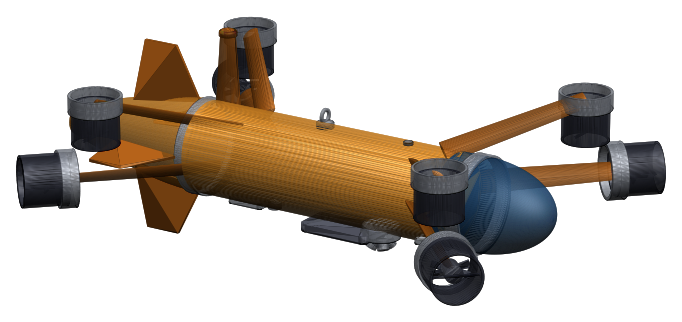
\includegraphics[width=0.66\linewidth]{../cad/varuna_hero_plain.png}
\end{center}

\vspace{-3mm}
\begin{center}\small
\begin{tabular}{@{}lc@{\hspace{6mm}}lc@{}}
\toprule
Station keeping envelope & \SI{\hydroEnvCad}{\metre\per\second} &
Navigation error, no external fix & \SI{\repNavMeanMean}{\metre} mean of \repRuns{} \\
Autonomous mission flown & \SI{\misPath}{\metre},
\SI{\misDurationMin}{min} & Bathymetric map error &
\SI{\repMapRmseMean}{\metre} \\
On a RISC-V flight computer & \SI{\hilNavMean}{\metre} &
Endurance, slack to design current & \enHoursCalm{} to
\SI{\enHoursSite}{\hour} \\
Depth rating & \SI{\structDepth}{\metre} &
Parts cost, one airframe & \SI{\bomLakh}{} lakh INR \\
\bottomrule
\end{tabular}
\end{center}

\section*{Why the usual platform will not do this}

An open frame vehicle of the class normally proposed for this role holds
station only to \SI{0.96}{\metre\per\second}. At the design current it is
swept away and no controller can prevent it. The purpose designed faired hull
raises that to \SI{\hydroEnvCad}{\metre\per\second} on drag derived from its
own geometry.

Comparable imported survey vehicles do not close this gap either, for a
structural reason rather than a performance one: REMUS 100 and Iver3 are
transit survey torpedoes, a single propeller with control fins, which needs
forward speed for control authority and gives no lateral thrust. That is right
for long survey lines in open water. It cannot hold station over a scoured
pier and orbit it to measure the hole. VARUNA gives up depth, endurance and
half its drag budget to buy exactly that.

\section*{Technology readiness, per subsystem}

\begin{center}\small
\begin{tabular}{@{}p{0.27\linewidth}c p{0.56\linewidth}@{}}
\toprule
\textbf{Subsystem} & \textbf{TRL} & \textbf{Evidence} \\
\midrule
Autonomy: estimation, control, mission logic & 4 &
Runs on a RISC-V flight computer inside a
\SI{\boardBudget}{\milli\second} real-time budget for a complete
\SI{\hilSimTime}{\second} mission, driving a separate microcontroller over a
CRC checked link. \\
Actuator interface & 4 &
Eight hardware PWM channels generated on the target microcontroller from the
allocation's own output; \espMatched{} of \espEchoes{} echoes exact, measured
from the duty registers. \\
Acoustic perception & 4 &
Trained and evaluated on real sonar, not simulation.
\SI{\yoloTestMapFifty}{\percent} on a held out real test split. \\
Geometric detection, mapping & 3 &
Validated against simulated ground truth only. \\
Vehicle structure, hydrodynamics & 3 &
Verified parametric CAD, closed mass and stability budget, closed form depth
and drag analysis. Nothing has been in water. \\
\bottomrule
\end{tabular}
\end{center}

\newpage

\section*{What was actually demonstrated}

\textbf{The autonomy runs on flight hardware.} The complete
\SI{\hilSimTime}{\second} mission was executed with estimation, control and
the mission state machine on a RISC-V single board computer, driven by
simulated physics on a host that never gives the board ground truth. It
reached the end state with a navigation error of \SI{\hilNavMean}{\metre}
against \SI{\misNavMean}{\metre} in pure simulation, using
\SI{\boardComputeMean}{\milli\second} of its \SI{\boardBudget}{\milli\second}
budget per tick.

The host and the board agree on the trajectory to roughly one part in
\num{e12} over \hilTicks{} ticks. That is the signature of the same arithmetic
in the same order, not of two implementations that happen to behave alike.

\textbf{The allocation reaches an actuator.} Over the same mission the flight
computer commanded \espSent{} pulse width frames to an ESP32 generating eight
real \SI{50}{\hertz} channels. \espMatched{} echoes exactly reproduced a
commanded width, read back from the timer's duty registers. \espMismatch{}
frame did not. Zero CRC errors on either link.

\textbf{Submerged vehicles are found without training data.} All
\detVehicleLargeHit{} large vehicles and \detVehicleSmallHit{} small
vehicle in the modelled scene are located in every run, at
\SI{\repDetErrMean}{\metre} mean error, from bathymetry alone. That
reduces an unsearchable \SI{\detSurveyHa}{\hectare} box to roughly
\detContacts{} georeferenced contacts to dive.

\section*{What is not claimed}

\begin{itemize}[leftmargin=*,itemsep=1pt,topsep=2pt]
\item \textbf{No physical vehicle exists.} Hydrodynamic coefficients are
closed form estimates cross checked against the CAD geometry, agreeing to
\SI{21}{\percent} in axial drag. CFD, tow tank and a pressure test remain
required.
\item \textbf{The detector is a screening tool, not a classifier.} It raises
about \detFalsePerHa{} spurious contacts per hectare alongside the real ones,
and misses a flat deck slab in two runs of \detRuns{}.
\item \textbf{Not single fault tolerant for station keeping.} Losing one of
four horizontal thrusters halves surge and drops the holdable current to
\SI{\redDegraded}{\metre\per\second}. The remedy is priced:
\SI{\redThrustNeeded}{\newton} thrusters instead of \SI{120}{\newton}.
\item \textbf{Simulator pretraining does not transfer to real sonar.} Measured
and reported as a negative result rather than omitted.
\end{itemize}

\section*{Where the money goes, and why that matters}

One airframe costs \bomTotal{} USD in parts, about \SI{\bomLakh}{} lakh INR.
The distribution is the interesting part: the two acoustic instruments are
\SI{\bomAcousticsPct}{\percent} of it, and the hull, propulsion, power and the
entire autonomy stack together come to \num{\bomRest} USD.

The work in this proposal therefore runs on hardware costing a few hundred
dollars, and it is the part that is genuinely ours. Hulls, thrusters and
pressure housings are not difficult to buy or to copy; the autonomy that flies
a survey in zero visibility against a \SI{\siteCurrent}{\metre\per\second}
current is. That is where the effort has gone, and it is why the readiness
table above is strongest exactly where the value is.

\section*{What the funding buys}

Not more analysis. Water.

\begin{center}\small
\begin{tabular}{@{}p{0.16\linewidth}p{0.40\linewidth}p{0.38\linewidth}@{}}
\toprule
\textbf{Phase} & \textbf{Work} & \textbf{Evidence produced} \\
\midrule
Months 1 to 6 & CFD and tow tank validation; pressure test of the hull
section; indigenous thruster and housing sourcing &
Measured coefficients replacing the closed form estimates; a qualified depth
rating \\
Months 7 to 12 & Integrated vehicle; tank and reservoir trials; sonar and
doppler integration & Wet testing against surveyed targets \\
Months 13 to 24 & Instrumented river trials with an operational partner;
scour measurement against diver survey & Field data at operational current
and turbidity \\
\bottomrule
\end{tabular}
\end{center}

This is the transition from readiness level 4 to levels 5 and 6, and it is the
step where testing facilities and an operational partner change the timeline
more than funding alone would. The Corps of EME's testing support and
integration space map directly onto months 7 to 24.

\vspace{2mm}
{\color{accent}\rule{\linewidth}{0.6pt}}

{\small Every number in this brief is generated from the measured result files
by a script in the repository, and is the same value the full technical report
carries. The report, the simulator, the autonomy stack, the CAD and the
hardware bench are all in one repository, and every result reproduces from a
single command.}

\end{document}
